\documentclass{report}

\usepackage[utf8]{inputenc}
\usepackage[T1]{fontenc}
\usepackage[francais]{babel}
\usepackage{textcomp}
\usepackage{amssymb}
\usepackage{algorithm}
\usepackage{algorithmic}
\usepackage{lipsum}
\usepackage{listingsutf8}
\usepackage{xcolor}
\usepackage[top=2.5cm,bottom=2.5cm,right=2.5cm,left=2.5cm]{geometry}
\usepackage{graphicx}

\lstset
    {language=C,
    frame=L,
    xleftmargin=\parindent,
    columns=flexible,
    basicstyle=\ttfamily\small,
    inputencoding=utf8/latin1,
    breaklines=true,
    breakautoindent=true,
    commentstyle=\color{black},
    keywordstyle=\color{blue},
    stringstyle=\color{black},
    commentstyle=\itshape\color{green!20!black},
    tabsize=2,
    extendedchars=true,
    showspaces=false,
    showstringspaces=false,
    numbers=left,
    numberstyle=\tiny,}

\newenvironment{myindentpar}[1]%
    {\begin{list}{}%
             {\setlength{\leftmargin}{#1}}%
             \item[]%
     }
     {\end{list}}


\title{Compte rendu du TP2 de Structure de Données}
\author{\textsc{Laurent} Valentin, \textsc{Malrin} Vincent}

\begin{document}

\maketitle

\tableofcontents

\setcounter{chapter}{1}
\newpage
\section{Objet du TP}\label{objet}
Représentation d'un dictionnaire par une information arborescente (stockage lvh).

\section{Structure de données}\label{sdd}
Chaque cellule de la structure arborescente contient une valeur (lettre),
un pointeur vers le fils, et un pointeur vers le frère.
Chaque valeur n'apparait qu'une seule fois parmi ses frères, les lettres appartienant
à une même liste chaînée par le lien horizontal sont ordonnées par ordre alphabétique.
De plus, si une valeur est une majuscule, la suite des lettres depuis la racine jusqu'à cet
lettre est un mot et si un mot est dans le dictionnaire, il existe un chemin depuis
une racine jusqu'à une lettre en majuscule dont les valeurs des cellules forment ce mot.

\begin{small}
\begin{verbatim}

       --        --------------------     --------------------     -------------------
arbre*|  |----->| 'a' | fils | frere |-->| 'b' | fils | frere |-->| 'z' | null | null |
       --        --------------------     --------------------     -------------------
                          |                        |
                          \/                       \/
                        --------------------      -------------------
                       | 'b' | fils | frere |    | 'o' | null | null | 
                        --------------------      -------------------
                                 |
                                 \/
                               --------------------     --------------------
                              | 'a' | fils | frere |-->| 'i' | fils | frere |
                               --------------------     --------------------
                                        |                        |
                                        \/                       \/
                                       -------------------      --------------------
                                      | 'T' | null | null |    | 'm' | fils | frere |
                                       -------------------      --------------------


\end{verbatim}
\end{small}

\newpage
\section{Organisation du code source}\label{source}
\subsubsection{arbre.h}
C'est le fichier d'entête des fonctions sur les arbres.

\subsubsection{arbre.c}
Ce fichier contient les fonctions :
\begin{myindentpar}{2cm}
\begin{itemize}
    \item construction
    \item lecture\_abr
    \item liberation\_abr
    \item affichage\_abr
    \item insertion\_abr
\end{itemize}
\end{myindentpar}

\subsubsection{lifo.h}
C'est le fichier d'entête des fonctions sur les piles.

\subsubsection{lifo.c}
Ce fichier contient les fonctions :
\begin{myindentpar}{2cm}
\begin{itemize}
    \item empiler
    \item depiler
    \item init\_lifo
    \item lifo\_vide
    \item lifo\_pleine
    \item free\_lifo
    \item afficher\_lifo
    \item inversion\_pile
\end{itemize}
\end{myindentpar}

\subsubsection{fifo.h}
C'est le fichier d'entête des fonctions sur les files.

\subsubsection{fifo.c}
Ce fichier contient les fonctions :
\begin{myindentpar}{2cm}
\begin{itemize}
    \item emfiler
    \item defiler
    \item init\_fifo
    \item fifo\_vide
    \item fifo\_pleine
    \item free\_fifo
    \item afficher\_fifo
\end{itemize}
\end{myindentpar}

\subsubsection{chaine.h}
C'est le fichier d'entête des fonctions sur les chaines de caractères.

\subsubsection{chaine.c}
Ce fichier contient les fonctions :
\begin{myindentpar}{2cm}
\begin{itemize}
    \item verif\_chaine
    \item verif\_arguments
\end{itemize}
\end{myindentpar}

\newpage
\section{Codes Sources}\label{codes}
\subsection{Question 1 : Inversion d'une pile}

\subsubsection{EN TÊTE lifo.c : lifo.h}
\begin{small}
\lstinputlisting{../inversion/lifo.h}
\end{small}

\subsubsection{GESTION PILE : lifo.c}
\begin{small}
\lstinputlisting{../inversion/lifo.c}
\end{small}

\subsubsection{EN TÊTE fifo.c : fifo.h}
\begin{small}
\lstinputlisting{../inversion/fifo.h}
\end{small}

\subsubsection{GESTION FILE : fifo.c}
\begin{small}
\lstinputlisting{../inversion/fifo.c}
\end{small}

\subsubsection{MAIN INVERSION: main.c}
\begin{small}
\lstinputlisting{../inversion/main.c}
\end{small}

\subsubsection{MAKEFILE}
\begin{small}
\lstinputlisting[language=make]{../inversion/makefile}
\end{small}

\newpage
\subsection{Question 2,3 et 4 : Gestion du dictionnaire arborescent}

\subsubsection{EN TÊTE arbre.c : arbre.h}
\begin{small}
\lstinputlisting{../dico/arbre.h}
\end{small}

\subsubsection{GESTION ARBRE : arbre.c}
\begin{small}
\lstinputlisting{../dico/arbre.c}
\end{small}

\subsubsection{EN TÊTE chaine.c : chaine.h}
\begin{small}
\lstinputlisting{../dico/chaine.h}
\end{small}

\subsubsection{GESTION CHAINE : chaine.c}
\begin{small}
\lstinputlisting{../dico/chaine.c}
\end{small}

\subsubsection{EN TÊTE lifo.c : lifo.h}
\begin{small}
\lstinputlisting{../dico/lifo.h}
\end{small}

\subsubsection{GESTION PILE : lifo.c}
\begin{small}
\lstinputlisting{../dico/lifo.c}
\end{small}

\subsubsection{MAIN DICO: main.c}
\begin{small}
\lstinputlisting{../dico/main.c}
\end{small}

\subsubsection{MAKEFILE}
\begin{small}
\lstinputlisting[language=make]{../dico/makefile}
\end{small}

\subsection{Script de tests : tests\_sdd.sh}
\begin{small}
\lstinputlisting[language=bash]{../tests_sdd.sh}
\end{small}

\newpage
\section{Jeux de tests}
\subsection{Cas à tester}
\subsubsection{Inversion de pile (Question 1)}
Cas à tester :
\begin{myindentpar}{2cm}
\begin{enumerate}
    \item Cas de chaine non valide (pour la lecture)
    \item Cas caractère unique
    \item Cas général
\end{enumerate}
\end{myindentpar}

\subsubsection{Validité des arguments du programme}
Cas à tester :
\begin{myindentpar}{2cm}
\begin{enumerate}
    \item Validité du fichier
    \item Validité de l'écriture parenthésée
    \item Validité des mots à insérer
\end{enumerate}
\end{myindentpar}

\subsubsection{Lecture et affichage (Question 2 et 3)}
Cas à tester :
\begin{myindentpar}{2cm}
\begin{enumerate}
    \item Cas arbre vide
    \item Cas arbre atomique
    \item Cas général
\end{enumerate}
\end{myindentpar}

\subsubsection{Insertion (Question 4)}
Cas à tester :
\begin{myindentpar}{2cm}
\begin{enumerate}
    \item Cas arbre vide
    \item Cas arbre atomique
        \begin{itemize}
            \item Cas insertion avant les frères
            \item Cas insertion apres les frères
            \item Cas insertion fils
        \end{itemize}
    \item Cas général
        \begin{itemize}
            \item Cas insertion avant les frères
            \item Cas insertion avant les frères (sans fils)
            \item Cas insertion entre les frères
            \item Cas insertion entre les frères (sans fils)
            \item Cas insertion apres les frères
            \item Cas insertion apres les frères (sans fils)
            \item Cas insertion fils
            \item Cas insertion d'un mot inclu
            \item Cas insertion d'un mot déjà présent
            \item Cas insertion sur une cellule sans frère (après)
            \item Cas insertion sur une cellule sans frère (après)
            \item Cas insertion avant racine
            \item Cas insertion apres racine
        \end{itemize}
    \end{enumerate}
\end{myindentpar}

\newpage
\subsection{Fichiers en entrée}

\subsubsection{Test de listes vides : abr\_vide.txt}
\lstinputlisting{../dico/abr_vide.txt}

\subsubsection{Test de cellule unique : abr\_atome.txt}
\lstinputlisting{../dico/abr_atome.txt}

\subsubsection{Test du cas général : abr\_verbe.txt}
\lstinputlisting{../dico/abr_verbe.txt}

\newpage
\subsection{Execution}
\subsubsection{Inversion (Question 1)}
\begin{itemize}
    \item Cas de chaine non valide : \./inversion/inversion
\vspace{0.5cm}
\lstinputlisting{../tests/tests_inversion1.txt}
\vspace{0.5cm}

    \item Cas caractère unique : \./inversion/inversion a
\vspace{0.5cm}
\lstinputlisting{../tests/tests_inversion2.txt}
\vspace{0.5cm}

    \item Cas général : \./inversion/inversion dcba
\vspace{0.5cm}
\lstinputlisting{../tests/tests_inversion3.txt}
\vspace{0.5cm}
\end{itemize}

\newpage
\subsubsection{Validité des arguments}
\begin{itemize}

    \item Validité du fichier : \./dico/dico inconnu.txt
\vspace{0.5cm}
\lstinputlisting{../tests/tests_finvalide.txt}
\vspace{0.5cm}

    \item Validité de l'écriture parenthésée 1 : \./dico/dico dico/abr\_err1.txt
\vspace{0.5cm}
\lstinputlisting{../tests/tests_err1.txt}
\vspace{0.5cm}

    \item Validité de l'écriture parenthésée 2 : \./dico/dico dico/abr\_err2.txt
\vspace{0.5cm}
\lstinputlisting{../tests/tests_err2.txt}
\vspace{0.5cm}

    \item Validité de l'écriture parenthésée 3 : \./dico/dico dico/abr\_err3.txt
\vspace{0.5cm}
\lstinputlisting{../tests/tests_err3.txt}
\vspace{0.5cm}

    \item Validité de l'écriture parenthésée 4 : \./dico/dico dico/abr\_err4.txt
\vspace{0.5cm}
\lstinputlisting{../tests/tests_err4.txt}
\vspace{0.5cm}

    \item Validité de l'écriture parenthésée 5 : \./dico/dico dico/abr\_err5.txt
\vspace{0.5cm}
\lstinputlisting{../tests/tests_err5.txt}
\vspace{0.5cm}

    \item Validité des chaines à insérer : \./dico/dico dico/abr\_vide.txt rien arbre7 @rbre arbré
\vspace{0.5cm}
\lstinputlisting{../tests/tests_err6.txt}
\vspace{0.5cm}
\end{itemize}

\newpage
\subsubsection{Lecture et Affichage (Question 3)}
\begin{itemize}

    \item Lecture -> Cas arbre vide : \./dico/dico dico/abr\_vide.txt
\vspace{0.5cm}
\lstinputlisting{../tests/tests_aff0.txt}
\vspace{0.5cm}

\begin{figure}[p]
    \caption{\label{abr_vide} Structure crée à partir de abr\_vide.txt}
   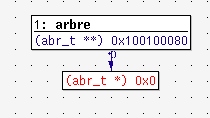
\includegraphics[scale=0.60]{./abr_vide.png}
\end{figure}

    \item Lecture -> Cas arbre atomique : \./dico/dico dico/abr\_atome.txt
\vspace{0.5cm}
\lstinputlisting{../tests/tests_aff1.txt}
\vspace{0.5cm}

\begin{figure}[p]
    \caption{\label{abr_atome} Structure crée à partir de abr\_atome.txt}
   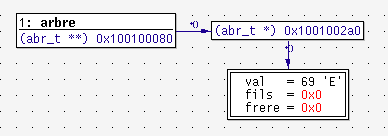
\includegraphics[scale=0.60]{./abr_atome.png}
\end{figure}

    \item Lecture -> Cas général : \./dico/dico dico/abr\_verbe.txt
\vspace{0.5cm}
\lstinputlisting{../tests/tests_aff2.txt}
\vspace{0.5cm}

\begin{figure}[p]
    \caption{\label{abr_verbe} Structure crée à partir de abr\_verbe.txt}
   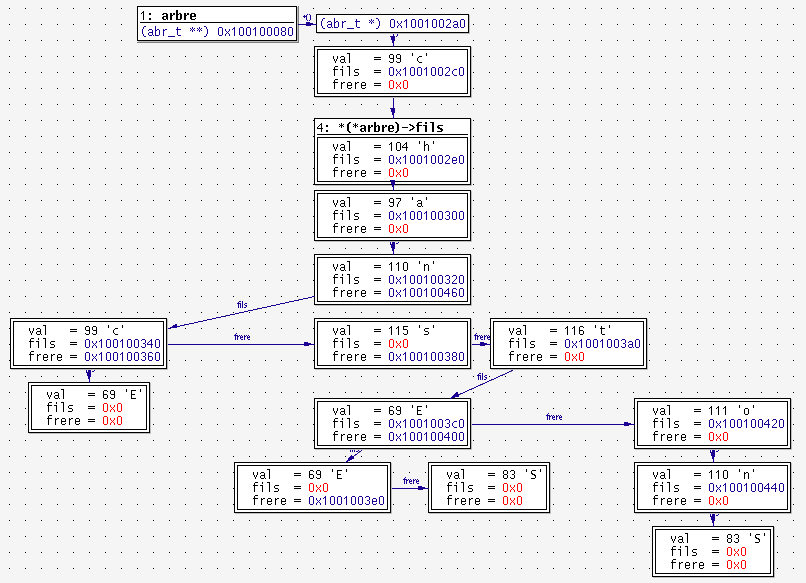
\includegraphics[scale=0.60]{./abr_verbe.png}
\end{figure}

\end{itemize}

\newpage
\subsubsection{Insertion (Question 4)}
\begin{itemize}

    \item Insertion -> Cas arbre vide : \./dico/dico dico/abr\_vide.txt abricoT
\vspace{0.5cm}
\lstinputlisting{../tests/tests_vide.txt}
\vspace{0.5cm}

    \item Insertion arbre atomique -> frere avant: \./dico/dico dico/abr\_atome.txt ah
\vspace{0.5cm}
\lstinputlisting{../tests/tests_atome1.txt}
\vspace{0.5cm}

    \item Insertion arbre atomique -> frere apres: \./dico/dico dico/abr\_atome.txt oh
\vspace{0.5cm}
\lstinputlisting{../tests/tests_atome2.txt}
\vspace{0.5cm}

    \item Insertion arbre atomique -> fil: \./dico/dico dico/abr\_atome.txt eh
\vspace{0.5cm}
\lstinputlisting{../tests/tests_atome3.txt}
\vspace{0.5cm}
\end{itemize}

\begin{enumerate}
    \item Insertion -> Avant les freres : \./dico/dico dico/abr\_verbe.txt chanta
\vspace{0.5cm}
\lstinputlisting{../tests/tests_insert1.txt}
\vspace{0.5cm}

    \item Insertion -> Avant les freres (sans fils) : \./dico/dico dico/abr\_verbe.txt chantea
Ce mot ne veut rien dire, c'est juste pour le test.
\vspace{0.5cm}
\lstinputlisting{../tests/tests_insert1bis.txt}
\vspace{0.5cm}

    \item Insertion -> Entre les freres : \./dico/dico dico/abr\_verbe.txt chantier
\vspace{0.5cm}
\lstinputlisting{../tests/tests_insert2.txt}
\vspace{0.5cm}

    \item Insertion -> Entre les freres (sans fils) : \./dico/dico dico/abr\_verbe.txt chanter
\vspace{0.5cm}
\lstinputlisting{../tests/tests_insert2bis.txt}
\vspace{0.5cm}

    \item Insertion -> Apres les freres : \./dico/dico dico/abr\_verbe.txt chans
\vspace{0.5cm}
\lstinputlisting{../tests/tests_insert3.txt}
\vspace{0.5cm}

    \item Insertion -> Apres les freres (sans fils) : \./dico/dico dico/abr\_verbe.txt chant
\vspace{0.5cm}
\lstinputlisting{../tests/tests_insert3bis.txt}
\vspace{0.5cm}

    \item Insertion -> fils : \./dico/dico dico/abr\_verbe.txt chansons
\vspace{0.5cm}
\lstinputlisting{../tests/tests_insert4.txt}
\vspace{0.5cm}

    \item Insertion -> Mot inclu : \./dico/dico dico/abr\_verbe.txt chant
\vspace{0.5cm}
\lstinputlisting{../tests/tests_insert5.txt}
\vspace{0.5cm}

    \item Insertion -> Mot déjà présent : \./dico/dico dico/abr\_verbe.txt chantons
\vspace{0.5cm}
\lstinputlisting{../tests/tests_insert6.txt}
\vspace{0.5cm}

    \item Insertion -> Cellule sans frère (après) : \./dico/dico dico/abr\_verbe.txt chartres
\vspace{0.5cm}
\lstinputlisting{../tests/tests_insert7.txt}
\vspace{0.5cm}

    \item Insertion -> Cellule sans frère (avant) : \./dico/dico dico/abr\_verbe.txt charles
\vspace{0.5cm}
\lstinputlisting{../tests/tests_insert8.txt}
\vspace{0.5cm}

    \item Insertion -> Avant racine : \./dico/dico dico/abr\_verbe.txt bavarde
\vspace{0.5cm}
\lstinputlisting{../tests/tests_insert9.txt}
\vspace{0.5cm}

    \item Insertion -> Après racine : \./dico/dico dico/abr\_verbe.txt discute
\vspace{0.5cm}
\lstinputlisting{../tests/tests_insert10.txt}
\vspace{0.5cm}

    \item Insertion -> Fils racine : \./dico/dico dico/abr\_verbe.txt calvitie
\vspace{0.5cm}
\lstinputlisting{../tests/tests_insert11.txt}
\vspace{0.5cm}
\end{enumerate}

\newpage
\subsubsection{Libération mémoire}
\begin{itemize}

    \item Valgrind -> DICO sans argument : valgrind \./dico/dico
\vspace{0.5cm}
\lstinputlisting{../tests/tests_free0.txt}
\vspace{0.5cm}

    \item Valgrind -> DICO : valgrind \./dico/dico dico/abr\_verbe.txt zorro
\vspace{0.5cm}
\lstinputlisting{../tests/tests_free1.txt}
\vspace{0.5cm}

    \item Valgrind -> INVERSION : valgrind \./inversion/inversion dcba
\vspace{0.5cm}
\lstinputlisting{../tests/tests_free2.txt}
\vspace{0.5cm}
\end{itemize}


\end{document}
